\section{文字功能}

\subsection{FreeGLUT 字型}

文字物件可以使用 FreeGLUT 的 Bitmap 與 Stroke 字型；Renderer 會處理 baseline，以及 Stroke 字型和 Canvas 相反的 Y 軸方向。這些內建字型主要用來顯示 ASCII。

\subsection{Text Object 與文字輸入}

選擇 Text tool 並點擊 Canvas 後，程式會開啟 Modal Input Dialog。只有在使用者確認文字後，才會建立 TextObject 並加入 Scene；如果取消輸入，Scene 不會留下空的文字物件。Dialog 只負責收集字串，實際修改 Document 的工作仍由 PaintWindow 完成。

輸入框內部以 Unicode code point 為編輯單位，對外仍使用 UTF-8 字串，因此 Backspace、Delete 與方向鍵不會切斷中文字的 bytes。FreeGLUT 的一般 keyboard callback 只能直接提供單一 byte，所以程式另提供反引號加四位十六進位數字的測試輸入，例如 \lstinline|`4f60| 會輸入「你」。Caret 與 UTF-8 bytes 的完整對應見附錄~\ref{app:gfnt}。

\begin{figure}[tbp]
    \centering
    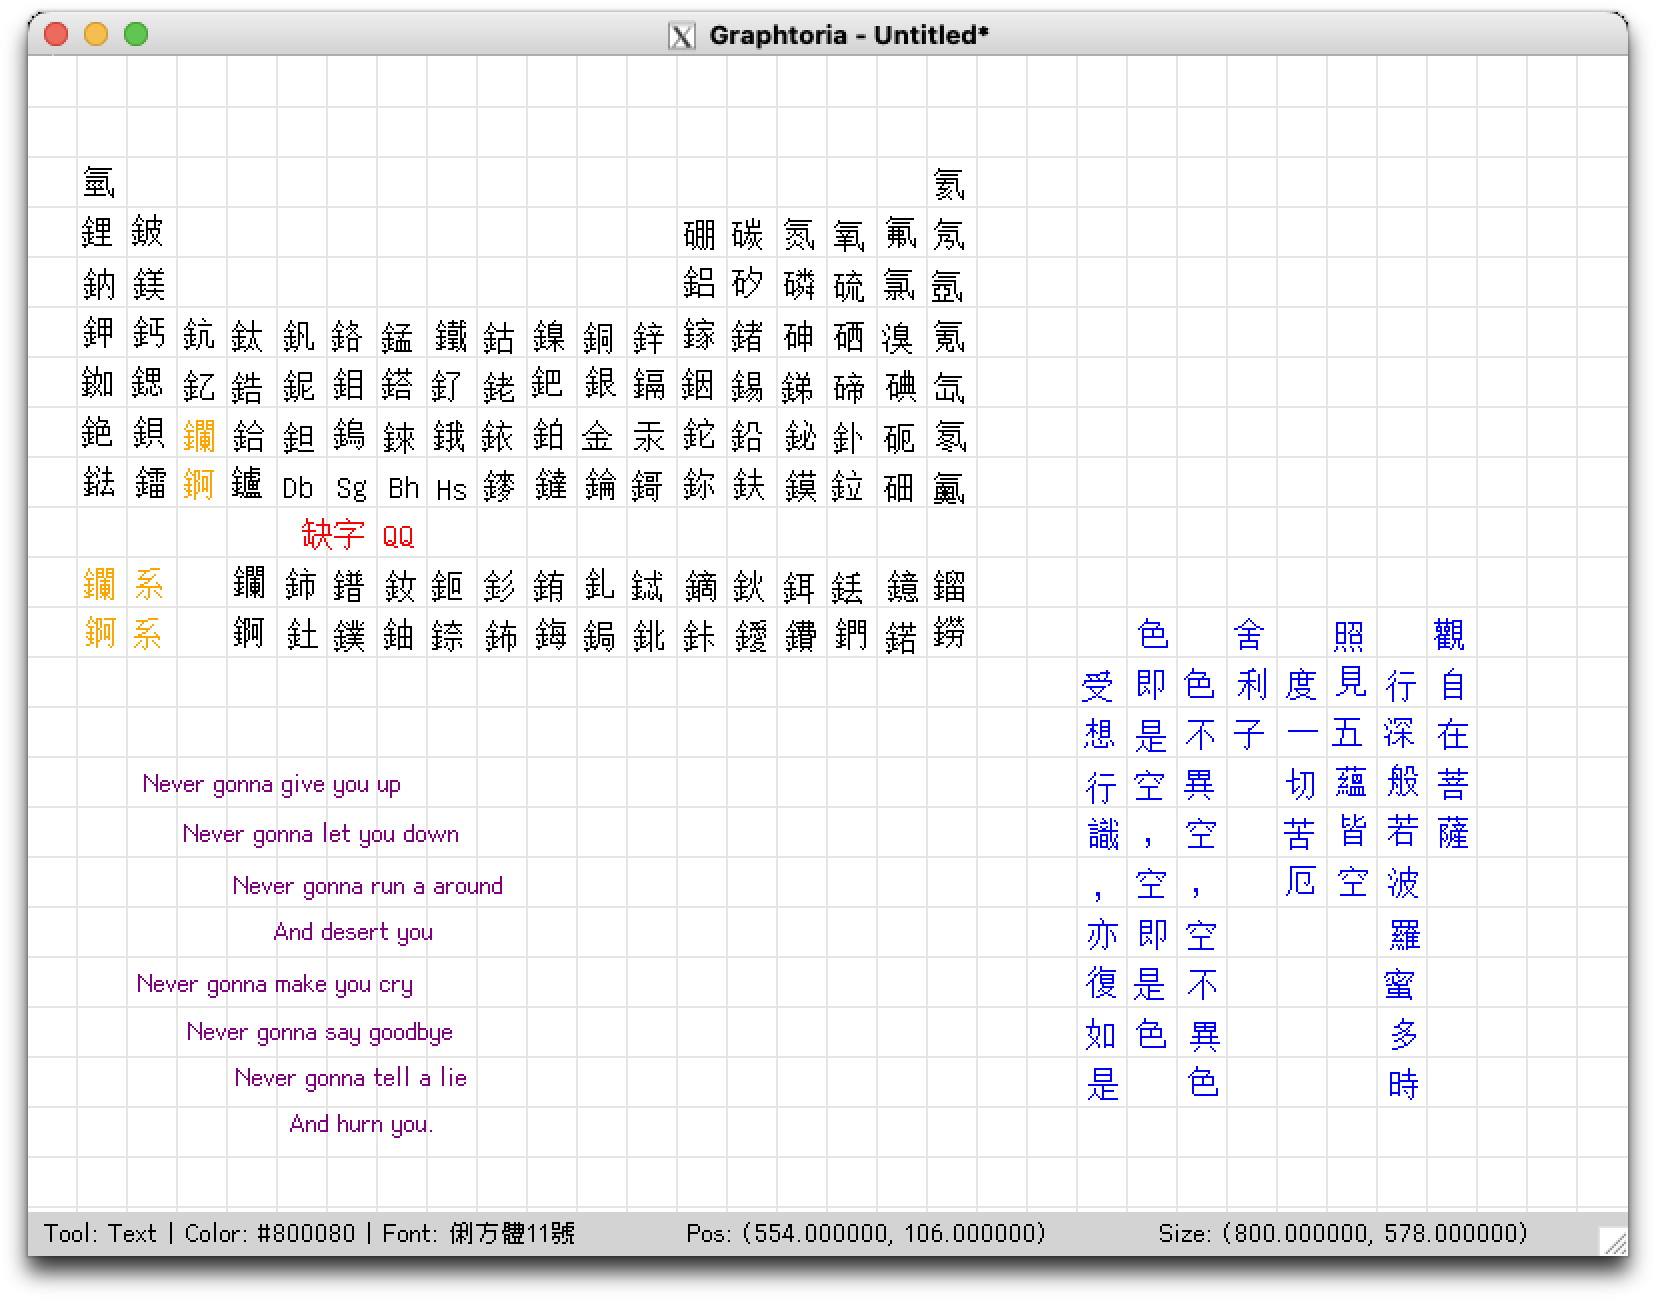
\includegraphics[width=.68\textwidth]{docs/figures/ch05_gfnt-chinese-output.png}
    \caption{GFNT 在程式中測試多個中文字形的實際輸出結果}
    \label{fig:text-result}
\end{figure}

圖~\ref{fig:text-result} 是從程式實際輸出的圖片裁切而成，可確認多個中文字都能找到對應 Glyph，字元順序與基線也符合輸入內容。

\subsection{UTF-8 與中文字元支援}

UTF-8 decoder 支援 1--4 byte sequence，遇到不合法輸入時以 \lstinline|U+FFFD| 取代。輸入框先將 UTF-8 轉成 code point 編輯，顯示時再重新編碼；TextRenderer 也使用相同流程逐字取得 glyph。

\subsection{自訂中文字型支援}

為了顯示 FreeGLUT 沒有涵蓋的中文字，我設計了 GFNT bitmap font。Renderer 從 UTF-8 取得 code point，查找 glyph 的尺寸、bearing、advance 與 bitmap，再組成 RGBA pixels 交給 OpenGL。執行期流程如圖~\ref{fig:gfnt-runtime}；binary layout、驗證與 fallback 規則收錄於附錄~\ref{app:gfnt}。

\begin{figure}[tbp]
    \centering
    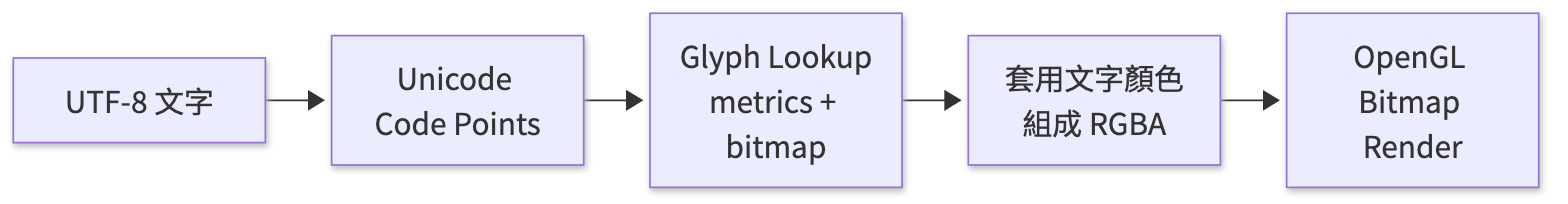
\includegraphics[width=.98\textwidth]{docs/figures/ch05_gfnt-runtime.png}
    \caption{GFNT 執行期文字渲染流程}
    \label{fig:gfnt-runtime}
\end{figure}
